\documentclass[10pt,conference]{IEEEtran}

\usepackage[utf8]{inputenc}
\usepackage{amsmath}
\usepackage{graphicx}
\usepackage{booktabs}
\usepackage{xcolor}
\usepackage{hyperref}


\begin{document}

\title{Predicting Coronary Heart Disease from the BRFSS Health Survey\\
with Regularized Linear Models}

\author{
  \IEEEauthorblockN{Rex Baseden, Michael Hanna, Tarek Hamad}
}

\maketitle

% ---------------------------------------------------------------------------
\section{Introduction}
Cardiovascular diseases are among the leading causes of death worldwide, and
early identification of people at risk can support prevention. We use the
Behavioral Risk Factor Surveillance System (BRFSS) telephone survey
to predict MICHD from lifestyle and health answers. The classes are
strongly imbalanced (approximately 9\% positives), so we evaluate with the F1 score and tune the decision threshold on out-of-fold predictions. We compare ridge
regression and (regularized) logistic regression, implemented from scratch in
NumPy, on top of a preprocessing pipeline based on one-hot encoding, median imputation and standardization.

% ---------------------------------------------------------------------------
\section{Data and Preprocessing}

\subsection{Dataset}
% Size, label balance, why accuracy is misleading.
The training set contains 328{,}135 respondents described by 321 numerically coded features, while the test set contains 109{,}379 respondents, about a third as many, whose labels are not provided. Only 9\% of training respondents are positive:
always predicting ``no MICHD'' reaches an accuracy of 91\% but an F1 of
0, which is why we use the F1 score of the positive class to measure how much we "learned" with our model.
Features are survey codes of three kinds: categorical answers (e.g.\ general
health from 1 to 5), counts (e.g.\ number of bad health days), and special
codes such as 77/99 (``don't know''/``refused'') or 88 (``none''). Many questions are only asked to subgroups, so missing values
are frequent.

\subsection{Feature processing}
% Be precise enough that someone could reimplement it (reproducibility).
\begin{enumerate}
  \item \textbf{Categorical vs.\ continuous.} A column with at most 10
    distinct values is one-hot encoded (a missing value gives all zeros).
    Other columns are kept as numbers, plus a binary indicator when they
    contain missing values.
  \item \textbf{Imputation and scaling.} Missing values are replaced by the
    training median; every feature is standardized to zero mean and unit
    variance; a bias column is added.
\end{enumerate}
This yields 1196 features. Steps 2 use no labels and is computed once on
the full training set; the statistics of step 3 are recomputed on the
training part of each cross-validation fold, so the validation fold never
influences them.

% ---------------------------------------------------------------------------
\section{Models and Training}

\subsection{Methods}
% Briefly: all six methods are implemented; which ones are used for prediction.
We implemented the six required methods in \texttt{implementations.py}. For
prediction we compare three of them, with labels mapped from
$\{-1,1\}$ to $\{0,1\}$:
ridge regression (normal equations, $\lambda=1e-5$),
logistic regression (gradient descent, $\gamma=0.1$, 1000 iterations),
and regularized logistic regression ($\lambda=1e-3$, same $\gamma$ and
iterations). Each model outputs a score $\tilde{x}^\top w$ per respondent.
% Optional implementation note (cut if space is short):
% Data is kept in float32; we made sure every operand is float32, since mixing
% with float64 made NumPy copy the full matrix at every gradient step
% (about 50x slower).

\subsection{Decision threshold}
Because positives are rare, a fixed cutoff is far from optimal for F1. We
choose the threshold that maximizes F1 on the pooled out-of-fold scores,
among 50 candidates: the 50th to 99th percentiles of the scores, i.e.\
labelling the top 1\% to 50\% as positive. For logistic regression this is
equivalent to thresholding the predicted probability.

% ---------------------------------------------------------------------------
\section{Experimental Setup}
We use 5-fold cross-validation with a fixed random split (seed 42). Each fold
model predicts its held-out fifth; the F1 is computed once on the pooled
out-of-fold predictions of all training respondents. Hyperparameters are selected by cross-validation only; the final model is
retrained on all training data and the selected threshold is applied to its
test scores.

% ---------------------------------------------------------------------------
\section{Results}

% Table 1: model comparison with baselines.
\begin{table}[t]
  \centering
  \caption{Model comparison (5-fold CV on the training set, AIcrowd test F1).}
  \label{tab:models}
  \begin{tabular}{lccc}
    \toprule
    Model & CV F1 & CV accuracy & Test F1 \\
    \midrule
    Always predict ``no'' & 0.000 & 0.91 & -- \\
    Ridge (tuned $\lambda=10^{-8}$)  & 0.4283 & 0.8695 & -- \\
    Logistic regression & 0.4378 & 0.8773 & 0.448 \\
    Reg.\ logistic regression & 0.4375 & 0.8772 & -- \\
    \bottomrule
  \end{tabular}
\end{table}

% Table 2: ablation study (explicitly required by the grading criteria).
\begin{table}[t]
  \centering
  \caption{Ablation study with logistic regression. Each row adds one step to
  the previous one.}
  \label{tab:ablation}
  \begin{tabular}{lcc}
    \toprule
    Configuration & \#features & CV F1 \\
    \midrule
    Raw features(missing set to 0)  & 321 & 0.1513 \\
    + standardization & 321 & 0.1794 \\
    + median imputation  & 321 & 0.4140 \\
    + one-hot encoding and missing indicators & 1190 & 0.4378 \\
    
    \bottomrule
  \end{tabular}
\end{table}

\begin{figure}[t]
  \centering
  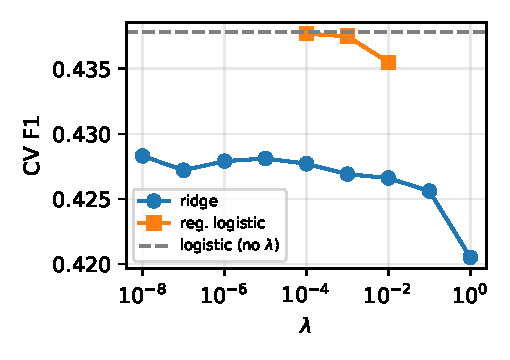
\includegraphics[width=\columnwidth]{../figures/f1_vs_lambda.pdf}
  \caption{Cross-validated F1 as a function of the regularization strength
  $\lambda$ for ridge and regularized logistic regression; the dashed line
  is logistic regression without regularization. The F1 is nearly constant
  for $\lambda \le 10^{-1}$, and regularization brings no gain for logistic
  regression.}
  \label{fig:lambda}
\end{figure}

% Describe the numbers in words: what improved, by how much, compared to noise.
Table~\ref{tab:models} compares the models. Table~\ref{tab:ablation} shows the effect of each step on the results. Fig.~\ref{fig:lambda} shows the
effect of $\lambda$.

% ---------------------------------------------------------------------------
\section{Discussion}
% Interpret, don't repeat the tables. Negative results are valuable too.

\textbf{Standardization.} The raw features span very different scales:
small answer codes, values such as BMI multiplied by 100, and large
bookkeeping values. With a single step size $\gamma$, gradient descent takes
steps that are far too large along the large-valued features and too small
along the others, so the optimization diverges or barely moves. The model is
then no better than predicting all respondents positive. Standardizing every
feature to zero mean and unit variance puts all directions on a comparable
scale, which is a prerequisite for gradient descent rather than a refinement.\\

\textbf{Median imputation.} Standardization alone helps little while missing
values are set to zero. For most features, zero is not a neutral value but
an extreme or impossible one (no respondent has a BMI of zero, and most
answer codes start at 1), so every missing entry becomes an outlier that
dominates the gradient and distorts the learned weights. Replacing missing
values by the training median places these respondents in the middle of the
distribution, where they do not pull the model in an arbitrary direction.
The two steps are therefore complementary: standardization works even more once the filled values are sensible.\\

\textbf{One-hot encoding and missing indicators.} Most survey features are
categories stored as numbers. Kept as numbers, a linear model can only learn
one weight per question, assuming that each answer code has an effect
proportional to its value, which is meaningless for codes such as 7
(``don't know'') or 9 (``refused''). One-hot encoding gives each answer its
own weight. The missing indicators keep the information that a value was
imputed, which is informative here because many questions are only asked to
respondents who gave a specific earlier answer. This step improves how the
data is represented rather than whether the model can be trained at all,
which explains why its gain is smaller than that of the first two steps.

% ---------------------------------------------------------------------------
\section{Conclusion}

No time

% References may go on a 3rd page.
\begin{thebibliography}{1}
\bibitem{brfss}
Centers for Disease Control and Prevention, ``Behavioral Risk Factor
Surveillance System, 2015 survey data,''
\url{https://www.cdc.gov/brfss/annual_data/annual_2015.html}.

\bibitem{codebook}
Centers for Disease Control and Prevention, ``BRFSS 2015 codebook report,''
2016.
\end{thebibliography}

\end{document}